%-----------------------------------LICENSE------------------------------------%
%   This file is part of Mathematics-and-Physics.                              %
%                                                                              %
%   Mathematics-and-Physics is free software: you can redistribute it and/or   %
%   modify it it under the terms of the GNU General Public License as          %
%   published by the Free Software Foundation, either version 3 of the         %
%   License, or (at your option) any later version.                            %
%                                                                              %
%   Mathematics-and-Physics is distributed in the hope that it will be useful, %
%   but WITHOUT ANY WARRANTY; without even the implied warranty of             %
%   MERCHANTABILITY or FITNESS FOR A PARTICULAR PURPOSE.  See the              %
%   GNU General Public License for more details.                               %
%                                                                              %
%   You should have received a copy of the GNU General Public License along    %
%   with Mathematics-and-Physics.  If not, see <https://www.gnu.org/licenses/>.%
%------------------------------------------------------------------------------%

%   Use the standalone class for displaying the tikz image on a small PDF.
\documentclass[crop, tikz]{standalone}

%   Import the tikz package to use for the drawing.
\usepackage{tikz}

%   Load the arrows.meta library.
\usetikzlibrary{arrows.meta}

%   Begin the document.
\begin{document}

    %   Draw the picture.
    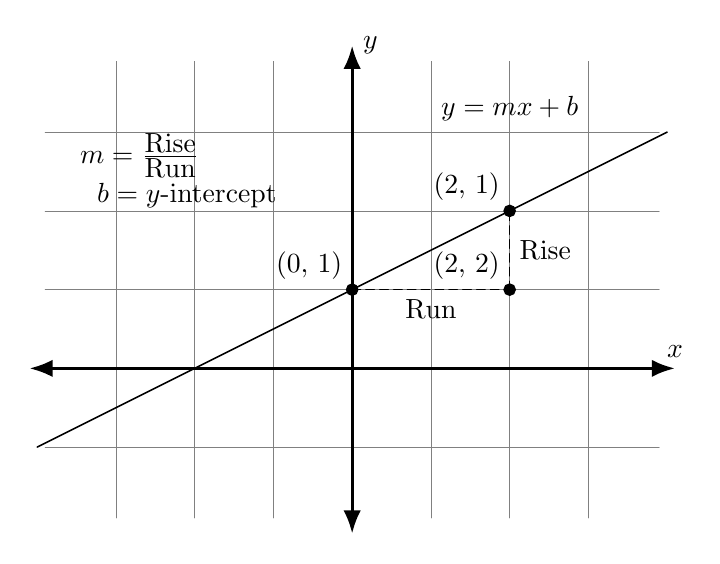
\begin{tikzpicture}[%
        >=Latex,
        line width=0.2mm,
        line cap=round,
    ]
        % Coordinates for various points.
        \coordinate (P1) at (0.0, 1.0);
        \coordinate (P2) at (2.0, 1.0);
        \coordinate (P3) at (2.0, 2.0);
        \coordinate (START) at (-4.0, -1.0);
        \coordinate (END) at (4.0, 3.0);
        \coordinate (m) at (-2.7, 2.7);
        \coordinate (b) at (-2.1, 2.2);
        \coordinate (y) at (2.0, 3.3);

        % Draw a grid.
        \draw[style=help lines] (-3.9, -1.9) grid (3.9, 3.9);

        % Axes.
        \begin{scope}[very thick]
            \draw[<->] (-4.1, 0.0) to (4.1, 0.0) node [above] {$x$};
            \draw[<->] (0.0, -2.1) to (0.0, 4.1) node [right] {$y$};
        \end{scope}

        % Draw the line.
        \draw (START) to (END);

        % Draw dots to mark various points.
        \draw[fill=black] (P1) circle (0.7mm) node [above left] {$(0,\,1)$};
        \draw[fill=black] (P2) circle (0.7mm) node [above left] {$(2,\,2)$};
        \draw[fill=black] (P3) circle (0.7mm) node [above left] {$(2,\,1)$};

        % Draw a triangle to indicate the slope of the line.
        \draw[densely dashed] (P1) to node [below] {Run} (P2);
        \draw[densely dashed] (P2) to node [right] {Rise} (P3);

        % Equations for the variables.
        \node at (m) {$m=\frac{\textrm{Rise}}{\textrm{Run}}$};
        \node at (b) {$b=y\textrm{-intercept}$};
        \node at (y) {$y=mx+b$};
    \end{tikzpicture}
\end{document}
